\documentclass[12pt,letterpaper]{article}
\usepackage[a4paper, total={7in, 10in}]{geometry}
\renewcommand{\familydefault}{\sfdefault}
\usepackage{graphicx}
\usepackage{helvet}
\usepackage{authblk}
\usepackage{hyperref}
\usepackage{amsmath} 
\usepackage{amssymb} 
\usepackage{orcidlink} 
\usepackage[super,comma,sort&compress]  
   {natbib}\bibliographystyle{numbered}
% \usepackage[right]{lineno} \linenumbers


\makeatletter
\renewcommand{\maketitle}{\bgroup\setlength{\parindent}{0pt}
\begin{flushleft}
  \textbf{\@title}
  
  \@author
\end{flushleft}\egroup}
\makeatother

%%%  Insert title below; leave date empty.

\title{Title is a maximum of 145 characters, including spaces, and avoids the use of jargon and uncommon abbreviations}
\date{}

%%%  Author first and last names should be spelled 
%%%  out in their entirety (do not abbreviate "J.H. 
%%%  Watson" unless this is how the author's name 
%%%  always appears). Middle initials are OK. Do 
%%%  not include titles, positions, or degrees.

%%%  Use numbered footnotes to indicate institutional 
%%%  affiliations. Authors may have multiple 
%%%  institutional affiliations, and affiliations 
%%%  may be shared among multiple authors.

%%%  After the institutional affiliations, numbered 
%%%  footnotes may be used to indicate an author's 
%%%  present address, equal contribution status, 
%%%  and/or senior author status. Corresponding 
%%%  authors may additionally include Twitter (X) 
%%%  handles as a means of contact.

%%%  The final numbered footnote should indicate 
%%%  which author is the lead contact (required). 
%%%  One author must be designated as the lead contact. 
%%%  There can be no more than one lead contact. 

%%%  Corresponding authors should be indicated with 
%%%  asterisks (*). Use 2 asterisks (**) for the 
%%%  second-listed corresponding author, 3 (***) for 
%%%  the third-listed, and so on. The lead contact 
%%%  must be a corresponding author. Additional 
%%%  authors may also serve as corresponding authors.

\author[1,5,\orcidlink{0000-0000-0000-0000}]{First Last}
\author[1,2,5]{First Middle Last}
\author[2,3]{First M.M. Last}
\author[3,*]{First Last, Jr.}
\author[3,4,6,7,8,**]{F. Middle Last}


%%%  Institutional affiliations should contain the 
%%%  following information at minimum: department(s)/
%%%  subunit(s), institution, city, state/region (if 
%%%  applicable), and country. 

\affil[1]{University A, London SW7 2AZ, UK}
\affil[2]{Department B, University B, Toronto, ON M5S 3H6, Canada}
\affil[3]{Division C, Department C, University C, Cambridge, MA, USA}

\affil[4]{Present address: 123 Sesame Street, New York, NY, USA}
\affil[5]{These authors contributed equally}
\affil[6]{Senior author}
\affil[7]{Twitter: @CorrespondingAuthor}
\affil[8]{Lead contact}

%%%  List only one email address per corresponding author.

\affil[*]{Correspondence: first.last.jr@university.edu}
\affil[**]{Correspondence: f.middle.last@university.edu}


\begin{document}

\maketitle

\section*{SUMMARY}

The summary (abstract) should consist of a single paragraph of 150 words or fewer.

\section*{KEYWORDS}

%%%  Include up to 10 keywords, separated by commas. 
%%%  Keywords entered in EM are not carried over; only 
%%%  keywords included in the main text will be used 
%%%  in the final article metadata. Please note that 
%%%  for some journals, keywords are chosen by the editors.

cell, press, LaTeX, template 

\section*{INTRODUCTION}

No subheadings, please. Use of abbreviations should be kept to a minimum, and nonstandard abbreviations should be defined when first used in the text.

\section*{RESULTS}

The results may be divided with subheadings. In our view, good subheadings convey information about the findings, so we encourage you to be specific. For example, "Factor X requires factor Y to function in process Z" is better than "Analysis of factors X and Y by approach Q." We recommend that you use similar language in your figure titles for clarity and structural harmony. Please do not use numbered subheadings. For some formats, ``results and discussion" may be combined under a single heading. 

\subsection*{Figures}

For initial submissions, figures and their titles and legends can be run-in with the text. For final submissions, the image files must be uploaded as separate files, one complete file per figure. The figure titles and legends should be placed toward the end of the main text, after the declaration of interests. Our typesetters will place the figures and their titles and legends appropriately based on your in-text citations.

\subsection*{Citations}

To cite/link to display items (figures and tables) and/or sections of the manuscript, simply write, for example, ``(Figure 1)" or ``see discussion." Our team will do the rest. Please note that we do not number sections or subsections.

To cite references, you may use the cite command, e.g., ``Recent articles in \textit{Matter} and \textit{Cell} \cite{wang2020conformational,king2002,cates1984statics}  have shown ..." or  ``Many interesting discoveries have been reported, \cite{radzihovsky1995new,kapoor2022leakage,hantke2018my,alcock2006} which ..." 

\subsection*{Equations}

Simple formulae should appear in line with the text whenever possible. You can write inline math by enclosing it between \verb|\(| and \verb|\)|, as in this example: \(x^2 + y^2 = z^2\). You can also enclose it between dollar signs (\texttt{\$}), as in this example: $E=mc^2$.

Larger, more complex formulae may appear on a new line, either by enclosing them between \verb|\[| and \verb|\]| or by using the \verb|displaymath| environment:

\[ x^n + y^n = z^n \]

\begin{displaymath}
\sqrt{x^2+1}
\end{displaymath}

If any equations or formulae need to be referred to or cited again later in the text, use the \verb|equation| environment to number them. Later, you can cite these as "Equation 1," "Equation 2," etc.

\begin{equation}
f(x) = \sum_{i=0}^{n} \frac{a_i}{1+x}
\end{equation}

\section*{DISCUSSION}

The discussion should explain the significance of the results and place them into a broader context. Subheadings are permitted.

\subsection*{Limitations of the study}

A "limitations" or "limitations of the study" subsection in the discussion is encouraged and may be required for some journals and some article formats.

\newpage





\noindent{The following Cell Press journals require most research articles to include their methods in a \textbf{METHODS} section, which should appear after the discussion: \textit{Cell Biomaterials}, \textit{Chem}, \textit{Chem Catalysis}, \textit{Cell Reports Physical Science}, \textit{Cell Reports Sustainability}, \textit{Device}, \textit{Joule}, \textit{Matter}, \textit{Newton}, \textit{One Earth}, and \textit{Patterns}. For all other Cell Press journals, please \textbf{delete} the contents of this page from the template and refer instead to \textbf{STAR Methods} on page 9.}

\section*{METHODS}

%%%  The methods (also/formerly called "experimental 
%%%  procedures") should appear 
%%%  immediately after the discussion. Subheadings 
%%%  may be customized. Please consult your handling 
%%%  editor if you have questions about what content 
%%%  should appear here. 


\subsection*{Custom methods subheading 1}
\subsection*{Custom methods subheading 2}
\subsection*{Custom methods subheading 3}
\subsection*{Custom methods subheading 4}

\newpage






%%%  The following components should appear after the 
%%%  methods. 
%%%  For journals using STAR Methods, these components 
%%%  should appear immediately after the discussion 
%%%  (after any "limitations" or "conclusions" subsection 
%%%  within the discussion).

\section*{RESOURCE AVAILABILITY}

%%%  The resource availability section is required 
%%%  for all research articles. This component 
%%%  has 3 subsections: "lead contact," "materials 
%%%  availability," and "data and code availability." 
%%%  All 3 subsections must be included, even if no 
%%%  unique materials were generated in the study. 
%%%  Do not edit or change the names of the subheadings. 
%%%  No other subheadings or text are allowed in the 
%%%  resource availability section.

\subsection*{Lead contact}

%%%  Authors are required to designate a lead contact, 
%%%  who will be responsible for communication with 
%%%  the journal before and after publication and is 
%%%  the arbiter of disputes, including concerns 
%%%  related to reagents or resource sharing. Only 
%%%  one author can be named the lead contact, and 
%%%  only the lead contact’s information may be 
%%%  provided in this section.

Requests for further information and resources should be directed to and will be fulfilled by the lead contact, Sally White (s.white@university.edu).

\subsection*{Materials availability}

%%%  This subsection must include a statement describing 
%%%  the availability of newly generated materials 
%%%  associated with the paper, including any conditions 
%%%  for access. If there are no newly generated materials 
%%%  associated with the paper, the statement should 
%%%  state this, e.g.: This study did not generate new 
%%%  materials.

Plasmids generated in this study have been deposited to [Addgene, name and catalog number or unique identifier].

\subsection*{Data and code availability}

%%%  All original research papers must include a 
%%%  comprehensive and accurate “data and code 
%%%  availability” statement within the “resource 
%%%  availability” component of the paper before it 
%%%  is accepted for publication. These statements 
%%%  are structured and consist of three bulleted 
%%%  components. Each component must be present.

\begin{itemize}
    \item Small-molecule crystallography data have been deposited at CCDC under the database identifier ABCDEF and are publicly available as of the date of publication. 1H NMR spectra have been deposited at Mendeley under the DOI 10.12345/a1b2c3d4e5f6g7.1 and are publicly available as of the date of publication. All other data reported in this paper will be shared by the lead contact upon request.
    \item All original code has been deposited at Zenodo under the DOI 10.56789/a1b2c3d4e5f6g7.1 and is publicly available as of the date of publication.\cite{georgios_rizos_2023_10253149}
    \item Any additional information required to reanalyze the data reported in this paper is available from the lead contact upon request.    
\end{itemize}


\section*{ACKNOWLEDGMENTS}

%%%  Use this section to acknowledge contributions 
%%%  from non-authors and list funding sources, 
%%%  including grant numbers.

This work was funded by [FUNDER] via grant [GRANT NO.]. The authors thank all members of the lab for their support.

\section*{AUTHOR CONTRIBUTIONS}

%%%  This component is required for most research papers. 
%%%  Mention each individual author with a statement 
%%%  outlining the contribution of each author to the work.

Conceptualization, S.C.P. and S.Y.W.; methodology, A.B., S.C.P., and S.Y.W.; investigation, M.E., A.N.V., N.A.V., S.C.P., and S.Y.W.; writing-–original draft, S.C.P. and S.Y.W.; writing-–review \& editing, S.C.P. and S.Y.W.; funding acquisition, S.C.P. and S.Y.W.; resources, M.E.V and C.K.B.; supervision, A.B., N.L.W., and A.A.D.

\section*{DECLARATION OF INTERESTS}

%%%  This component is required for all articles, even 
%%%  if the authors have no competing interests; if 
%%%  this is the case, insert "The authors declare no 
%%%  competing interests." Please refer to the 
%%%  declaration of interests policy: 
%%%  https://www.cell.com/declaration-of-interests

S.Y.W. is an employee and shareholder of COMPANY. M.E.V. is a founder of COMPANY and a member of its scientific advisory board.

\section*{DECLARATION OF GENERATIVE AI AND AI-ASSISTED TECHNOLOGIES}

%%%  If generative AI and AI-assisted technologies 
%%%  were used in the writing process, this must 
%%%  be disclosed in the paper. This declaration 
%%%  does not apply to the use of basic tools for 
%%%  checking grammar, spelling, references, etc. 
%%%  If you have nothing to disclose, please do not 
%%%  include this component.

During the preparation of this work, the author(s) used [NAME OF TOOL OR SERVICE] in order to [REASON]. After using this tool or service, the author(s) reviewed and edited the content as needed and take(s) full responsibility for the content of the publication.

\section*{SUPPLEMENTAL INFORMATION INDEX}

%%%  Supplemental information must be uploaded as 
%%%  separate files. In the main text, please list the 
%%%  files to be included in a brief index. For details, 
%%%  please review the supplemental information guidelines: 

%%%  Journals with a general "methods" section: 
%%%  http://www.cell.com/supplemental-information

%%%  Journals with STAR Methods: 
%%%  https://www.cell.com/STAR-supplemental-information

\begin{description}
  \item Figures S1-S5 and their legends in a PDF
  \item Table S1. A descriptive title for an Excel file that was too large to appear in the PDF
  \item Table S2. Another descriptive title for a different Excel file
  \item Data S1. Raw data on x, y, and z
\end{description}

\newpage





\section*{MAIN FIGURE TITLES AND LEGENDS}

%%%  At final submission, figure files MUST be 
%%%  provided separately as high-resolution image 
%%%  files. All of the panels for a figure should 
%%%  be in the same file. Figures should have 
%%%  clear labels/file names (Figure 1, Figure 2, 
%%%  etc.). 

%%%  Figure titles and legends should be placed 
%%%  at the end of the main text. You do not 
%%%  need to place the figures, nor their titles 
%%%  and legends, within the main text. While 
%%%  typesetting your article, our team will 
%%%  place each figure in the best location 
%%%  based on the final layout and on your 
%%%  figure citations, e.g., (Figures 1A and 1B). 

%%%  Please review the figure guidelines before 
%%%  submitting your final materials: 
%%%  https://www.cell.com/figureguidelines.

\noindent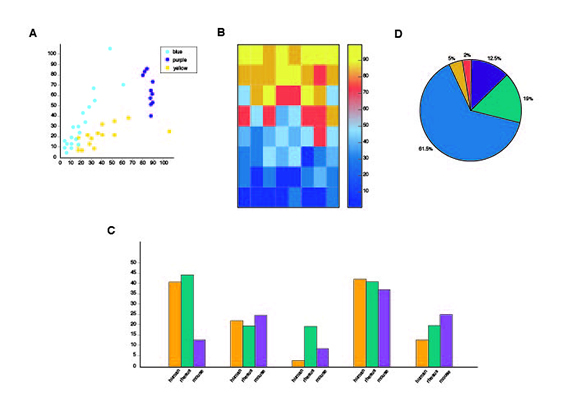
\includegraphics[width=0.85\linewidth]{Figure1.jpg}

\subsection*{Figure 1. A brief title that describes the entire figure without citing specific panels}

The figure legend can be all one paragraph and describe the images (A), graphs (B), and plots (C), etc., together.
\newline
(A) Or each panel or group of panels can be described separately, as shown here and below.
\newline
(B) Graph of X, Y, and Z.
\newline
(C and D) If panels are grouped like this, please explicitly describe each panel, e.g., “Images showing SEM (C) and TEM (D).”
\newline
Please define all scale and error bars, and please review the Cell Press figure guidelines before submission: \href{https://www.cell.com/figureguidelines}{https://www.cell.com/figureguidelines}. Example figure created by Cassie Comeau, Cell Press.

\newpage

\section*{MAIN TABLES, INCLUDING TITLES AND LEGENDS}

%%%  Whenever possible, we encourage you to submit 
%%%  your main-text tables as Microsoft Word documents, 
%%%  using Word's table function. This will ensure 
%%%  the best results during conversion. Tables 
%%%  should be numbered Table 1, Table 2, etc. and 
%%%  should not include subpanels (do not use Table 1A, 
%%%  1B, etc.). Give each table a brief descriptive 
%%%  title. Table legends are optional but encouraged. 
%%%  Footnotes (superscript lowercase letters) should 
%%%  be used where necessary to indicate some feature 
%%%  of the data; please do not use bold, italic, 
%%%  colored text, or shading for this purpose. Use 
%%%  separate cells, not line breaks or spaces, for 
%%%  all discrete data elements. Small embedded 
%%%  graphics with color are OK.

%%%  Like figures, all tables must be cited within 
%%%  the main text, and our typesetting team will 
%%%  place the tables within the typeset paper at 
%%%  the appropriate locations.


\subsection*{Table 1. A table with clear organization of data}

\begin{tabular}{|l | l | l | l|} 
 \hline
 \textbf{Column 1} & \textbf{Column 2} & \textbf{Column 3} & \textbf{Column 4} \\ [1ex] 
 \hline
 Row A\textsuperscript{a} & 6 & 87,837 & 787 \\ [1ex] 
 \hline
 Row B & 7 & 78 & 5,415 \\ [1ex] 
 \hline
 Row C & 545 & 778 & 7507 \\ [1ex] 
 \hline
 Row D & 545 & 18,744 & 7,560 \\ [1ex] 
 \hline
 Row E & 88 & 788 & 6,344 \\ [1ex] 
 \hline
\end{tabular}

\bigskip

The table legend (optional) follows the table itself. The legend should be used to provide additional info that relates to the table as a whole.

\textsuperscript{a}Footnotes can be used to provide additional info on specific content within the table, such as this footnote to the first row (row A). Do not use footnotes in the table title.

\textsuperscript{b}More footnotes

\newpage

%%%  REFERENCES: As of 2023, all Cell Press journals 
%%%  use Numbered (AMA) style. We recommend placing 
%%%  your references in the included "references.bib" 
%%%  file.


\bibliography{references}



\bigskip

%%%  In your References, please include only articles 
%%%  that are published (online publication and 
%%%  preprint servers are OK). Unpublished data, 
%%%  submitted and/or accepted manuscripts, abstracts, 
%%%  and personal communications should be cited within 
%%%  the text only ("unpublished data," "data not 
%%%  shown," "Alice Smith, personal communication") 
%%%  and not included in the references list. Personal 
%%%  communication should be documented by a letter 
%%%  of permission. Whenever possible, please make 
%%%  sure your .bib file has the complete author lists 
%%%  for each item (at minimum, the first 11 authors 
%%%  listed). 

\newpage






All Cell Press \textbf{life and medical science} journals, and the multidisciplinary journal \textbf{iScience}, use the \textbf{\href{https://www.cell.com/star-authors-guide}{STAR Methods}} format for reporting materials and methods. Other Cell Press journals use a non-structured \textbf{methods} format; for those journals, please \textbf{delete} the contents of this page from the template and refer instead to the \textbf{methods} template on page 3.

If you are publishing in a STAR Methods journal, please refer to the appropriate guide for authors:
\begin{itemize}
\item \textit{Cell} authors should download the guide for \textit{Cell} authors \href{https://www.cell.com/pb-assets/journals/research/cell/methods/Methods_Guide_Cell-1678470557763.pdf}{available here}
\item All other journal authors should use \href{https://www.cell.com/pb-assets/journals/research/cell/methods/Methods_Guide_general-1678470557763.pdf}{this version of the guide}
\end{itemize}


\section*{STAR METHODS}

%%%  The STAR Methods should appear in your main 
%%%  manuscript file after the figure legends, main 
%%%  table(s) and table legend(s).

\subsection*{Key resources table}

\textit{To create the KRT, please use the \href{https://star-methods.com}{KRT webform} or the \href{http://www.cell.com/pb-assets/journals/research/cell/methods/table-template1.docx}{Word template} and upload this file separately.}

\subsection*{Experimental model and study participant details}

%%%  Please list here under separate headings 
%%%  all the experimental models/study participants 
%%%  (animals, human participants, plants, microbe 
%%%  strains, cell lines, primary cell cultures) 
%%%  used in the study. For each model, provide 
%%%  information related to their species/strain, 
%%%  genotype, age/developmental stage, sex (and 
%%%  gender, ancestry, race, and ethnicity if 
%%%  reported for human studies), maintenance, 
%%%  and care, including institutional permission 
%%%  and oversight information for the studies 
%%%  the experimental animal/human participant 
%%%  study. The influence (or association) of sex, 
%%%  gender, or both on the results of the study 
%%%  must be reported. In cases where it cannot, 
%%%  authors should discuss this as a limitation 
%%%  to their research’s generalizability.

%%%  Please omit this component if your study does 
%%%  not use experimental models typical in the 
%%%  life sciences (e.g., if your study is 
%%%  computational or physical science research). 

\subsection*{Method details}

%%%  Please provide precise details of all the 
%%%  procedures in the paper (behavioral task, 
%%%  generation of reagents, biological assays, 
%%%  modeling, etc.) such that it is clear how, 
%%%  when, where, and why procedures were 
%%%  performed. We encourage authors to provide 
%%%  information related to the experimental 
%%%  design as suggested by NIH and ARRIVE 
%%%  guidelines (e.g., information about 
%%%  replicates, randomization, blinding, sample 
%%%  size estimation, and the criteria for 
%%%  inclusion and exclusion of any data or 
%%%  subjects).

\subsection*{Quantification and statistical analysis}

%%%  Please describe here all statistical analysis 
%%%  and software used. We ask authors to indicate 
%%%  in this component where all of the statistical 
%%%  details of experiments can be found (e.g., in 
%%%  the figure legends, figures, results, etc.), 
%%%  including the statistical tests used, exact 
%%%  value of n, what n represents (e.g., number 
%%%  of animals, number of cells, etc.), definition 
%%%  of center, and dispersion and precision 
%%%  measures (e.g., mean, median, SD, SEM, confidence 
%%%  intervals). Also, please summarize in this 
%%%  component how significance was defined, the 
%%%  statistical methods used to determine strategies 
%%%  for randomization and/or stratification, sample 
%%%  size estimation, and inclusion and exclusion 
%%%  of any data or subjects, as well as any methods 
%%%  used to determine whether the data met 
%%%  assumptions of the statistical approach.

\subsection*{Additional resources}

%%%  Please provide links to websites that provide 
%%%  further information relevant to the study 
%%%  (e.g., protocol download, troubleshooting 
%%%  forum, etc.). Clinical trial registry numbers 
%%%  and links should also be placed here. Please 
%%%  briefly describe the resource and its 
%%%  relevance for the paper. Please report this 
%%%  information as: “Description: URL.”

Cell.com homepage: https://www.cell.com
\newline Templates for Cell Press authors: https://www.cell.com/article-templates

%%%  ADDITIONAL MANUSCRIPT COMPONENTS:

%%%  Depending on the journal and the article 
%%%  type, you may be asked to upload the 
%%%  following as separate files: graphical 
%%%  abstract, highlights, eTOC blurb (In 
%%%  Brief), and/or other article components 
%%%  such as a "bigger picture" statement. 
%%%  These items are typically not required for 
%%%  initial submissions. Please refer to the 
%%%  journal's website, your acceptance 
%%%  letter, and/or the Final Files 
%%%  Requirements checklist to see if any of
%%%  these items are required (at any stage).


\end{document}
